\documentclass[a4paper,fleqn]{cas-sc}

% Elsevier CAS template; target journal: Simulation Modelling Practice and Theory.
\usepackage[T1]{fontenc}
\usepackage[utf8]{inputenc}
\usepackage[english]{babel}
\usepackage[authoryear]{natbib}
\usepackage{amsmath,amssymb}
\usepackage{graphicx}
\usepackage{tikz}
\usetikzlibrary{positioning,fit,arrows.meta}
\usepackage{booktabs}
\usepackage{array}
\usepackage{float}
\usepackage{xcolor}
\usepackage{microtype}
\microtypesetup{expansion=false}
\IfFileExists{xurl.sty}{\usepackage{xurl}}{\usepackage{url}}
\setlength{\emergencystretch}{3em}
\hyphenation{inter-community intra-community Gillespie}

\floatstyle{ruled}
\newfloat{algorithm}{tbp}{loa}
\floatname{algorithm}{Algorithm}
\floatstyle{plain}
\restylefloat{figure}
\restylefloat{table}

\newtheorem{proposition}{Proposition}
\newtheorem{corollary}{Corollary}
\newdefinition{remark}{Remark}
\newproof{proof}{Proof}

\newcommand{\ibar}{\bar{y}}
\newcommand{\sbar}{\bar{s}}
\newcommand{\Exp}{\mathrm{Exp}}
\newcommand{\Full}{\textup{\textsc{Full}}}
\newcommand{\TS}{\textup{\textsc{TwoScale}}}
\newcommand{\ind}{\mathbf{1}}
\newcommand{\eW}{e_{W}}

% Full-paper numbers for material not yet translated into this partial main.
\AtBeginDocument{
\newlabel{app:clique}{{A}{25}{}{}{}}
\newlabel{app:repro}{{C}{28}{}{}{}}
\newlabel{sec:discussion}{{7}{22}{}{}{}}
\newlabel{sec:res_descriptor}{{6.6}{20}{}{}{}}
\newlabel{sec:results}{{6}{15}{}{}{}}
}
\begin{document}
\let\WriteBookmarks\relax
\def\floatpagepagefraction{1}
\def\textpagefraction{.001}

\shorttitle{Two-scale stochastic simulation with aggregate inter-community coupling}
\shortauthors{Y. Kuryliak and M.T.M. Emmerich}

\title[mode=title]{Two-scale stochastic simulation of epidemics on community networks with aggregate inter-community coupling}

\author[1]{Yulian Kuryliak}[orcid=0000-0002-6600-2637]
\cormark[1]
\ead{yulian.a.kuryliak@lpnu.ua}
\affiliation[1]{organization={Institute of Computer Science and Information Technologies, Lviv Polytechnic National University},
            addressline={12 Stepan Bandera Street},
            city={Lviv},
            postcode={79000},
            country={Ukraine}}

\author[2]{Michael T. M. Emmerich}[orcid=0000-0002-7342-2090]
\ead{michael.t.m.emmerich@jyu.fi}
\affiliation[2]{organization={Faculty of Information Technology, University of Jyv\"askyl\"a},
            addressline={P.O. Box 35 (Agora)},
            city={Jyv\"askyl\"a},
            postcode={FI-40014},
            country={Finland}}

\cortext[1]{Corresponding author}

% Provisional abstract for checking the native SMPT front-matter layout.
\begin{abstract}
test 


test

test



test




test

test
\end{abstract}

\begin{keywords}
Stochastic simulation \sep Gillespie algorithm \sep Multiscale simulation \sep Community networks \sep Epidemic modelling \sep Approximation error
\end{keywords}

\maketitle
% English translation of the user's saved Ukrainian Sections 1--3.
% Original baseline: claude-version_merged_parallel_EN.tex.

%======================================================================
\section{Introduction}
\label{sec:introduction}

Epidemics spread at more than one scale. Inside a community, infection may pass through a detailed network of contacts between people \citep{keeling2005,pastorsatorras2015,kiss2017}. Between communities, the available data are often much less detailed. For example, they may give only passenger numbers, commuting flows, or a weighted link between two places \citep{balcan2009,barbosa2018human}. We therefore need a model that can use a detailed network inside each community and simpler data between communities.

This situation is common in practice. A local contact network may be observed, reconstructed, or generated to match known properties such as clustering and mean shortest-path length \citep{eubank2004,danon2011}. In contrast, links between communities may be known only through transport, migration, commuting, or mobile-phone data \citep{barbosa2018human,chang2021}. Such data can tell us the total strength of connection between two communities, but not which people form the connection. We may therefore know the total coupling without knowing the bridge nodes or their infection states.

If every contact is known, a continuous-time Markov chain (CTMC) can describe the epidemic, and the Gillespie method can simulate it exactly \citep{gillespie1977exact,gibson2000}. Efficient methods are also available for temporal, large, and sparse networks \citep{vestergaard2015,kuryliak2025simulating}. However, these methods still need the individual contacts that may transmit infection. Metapopulation models use aggregate flows between communities, but usually also replace the detailed local network by counts of people in different states \citep{colizza2007reaction,colizza2008,balcan2010modeling,ajelli2010}. Our problem lies between these two cases: we want to keep node-level stochastic spread inside every community while using only aggregate information between communities.

The idea of a two-scale simulator was presented in an earlier conference paper \citep{kuryliak2025towards}. It runs a separate local simulator for each community. The macro layer uses the current community states and connection weights to generate infections arriving from another community. In this article, we describe the method in detail and study its approximation error. In particular, we examine what is lost when real cross-community edges and their endpoints are replaced by the total connection weight, and an imported infection is placed on a randomly selected susceptible node.

Our main question is: when is this aggregate connection sufficient to reproduce the quantity of interest in the full-network CTMC? We study infection arrival times, their distributions, and whether transmission is possible through the real contacts. Similar arrival times do not guarantee a possible transmission route: the two-scale model can infect another community while all real bridge nodes in the source community are still susceptible. To test this, we use synthetic networks in which every contact is known. Full-network Gillespie simulation receives the whole network, whereas the two-scale method receives only the local networks and the total weights of the cross-community connections.

This article makes four contributions.
\begin{enumerate}
\item We describe how the simulator works: each community is simulated separately, and a shared scheduler determines infections between them. We explain how it coordinates the local simulators on time intervals of fixed length (Section~\ref{sec:method}, Algorithm~\ref{alg:scheduler}).
\item We show which network the method simulates exactly. The ideal process is exact for a \emph{surrogate network with uniform inter-community connections}: for each connected community pair, every node in one community is connected to every node in the other, and the total coupling weight is distributed equally among these node pairs (Proposition~\ref{prop:surrogate}). We then identify the sources of error and analyse a single export of infection (Proposition~\ref{prop:ordering}).
\item We compare the two-scale method with full-network Gillespie simulation for transmission to one neighbouring community and for spread along chains of communities. We measure differences using the relative shift in the median time of first infection and the Wasserstein distance between the distributions of these times (Sections~\ref{sec:design} and~\ref*{sec:results}).
\item We propose an empirical indicator of accuracy for our benchmarks. It compares the spread of infection times inside a community with the typical transmission time through one cross-community edge (Section~\ref*{sec:res_descriptor}).
\end{enumerate}

We consider susceptible--infected (SI) dynamics on static synthetic networks and use one fixed synchronisation step. Section~\ref{sec:related} explains the relation to earlier methods. Section~\ref{sec:method} describes the simulator. Section~\ref{sec:analysis} explains what the aggregate interface preserves and loses. Sections~\ref{sec:design} and~\ref*{sec:results} present the experiments and results. Section~\ref*{sec:discussion} discusses use, cost, and limitations.


%======================================================================
\section{Related work}
\label{sec:related}

\paragraph{Simulation of stochastic events.}
Gillespie's direct method draws the next event and its time from the current event rates \citep{gillespie1977exact}. The next reaction method keeps a separate clock for each possible event \citep{gibson2000}. Both methods are exact for the CTMC they simulate. When an event rate changes with time, its rate can be accumulated until it reaches a random threshold \citep{ethier1986}. \citet{anderson2007} used this idea for systems with time-dependent rates and delays. Our macro clock uses the same idea, but its rate changes because the local epidemic states change. Network simulators can save work by updating only the rates affected by the latest event \citep{vestergaard2015,kuryliak2025simulating}. Our local simulators use the implementation of \citet{kuryliak2025simulating}.

Some multiscale methods speed up chemical-reaction models by approximating reactions that occur much faster than others \citep{haseltine2002,cao2005slow}. Our method removes a different kind of detail. It keeps the local infection events, but does not know which individual cross-community edges are currently able to transmit. Even so, the relative speeds of local spread and cross-community transmission help explain its error.

\paragraph{Models with several communities.}
Metapopulation models represent each subpopulation by counts of people in different states and connect the subpopulations by mobility flows. They have been used to study global spread and the conditions for invasion \citep{colizza2007reaction,colizza2008,balcan2009,balcan2010modeling}. Detailed mobility data can also be combined with local transmission models \citep{chang2021}. Agent-based models instead represent individuals throughout the model \citep{eubank2004,kerr2021}. \citet{ajelli2010} compared these two broad approaches. The method studied here keeps individual nodes and contacts inside each community, but replaces the unknown individual contacts between communities by one aggregate stochastic interface.

\paragraph{Two levels of mixing and co-simulation.}
Some epidemic models combine contacts in small local groups with uniform mixing at a wider level \citep{ball1997}. Our surrogate network with uniform inter-community connections is related to this idea, but uniform mixing is used only between connected pairs of communities, and its strength is set by their aggregate weight.

The implementation also has features of co-simulation. In co-simulation, separate subsystem solvers move forward on a shared time grid and exchange a limited amount of information \citep{gomes2018cosim}. Here, the local community simulators are those subsystems. They send their infected and susceptible counts to the macro layer. The macro layer uses these data to generate the time of a cross-community infection and select the receiving community and target node. The local simulators can therefore remain black boxes for the scheduler. In this implementation, the exchanged data are used to create random infection events.


%======================================================================
\section{The two-scale simulation method}
\label{sec:method}

The experiments use one implementation of the two-scale simulator, in which the local simulators exchange information with the macro scheduler at fixed time intervals. To understand its error, we also consider a process with the same rates but exact timing of every event. We call this theoretical description the \emph{ideal process}. It separates the error caused by changing the network from the additional error caused by the time grid. The ideal process is exact for the surrogate network with uniform inter-community connections defined later; this does not make it exact for the original physical network. Below, we explain the reference model, the available data, and the steps of the implemented simulator.

\subsection{Full-network reference model}
\label{sec:reference}

Let $G=(V,E)$ be the contact network. Its nodes are divided into $M$ non-overlapping communities:
\begin{equation}
\label{eq:partition}
V=V_1\cup V_2\cup\cdots\cup V_M,
\qquad N_i=|V_i|.
\end{equation}
Here, $V_i$ is the node set of community $i$, and $N_i$ is its size. We write $E_{ii}$ for contacts inside community $i$ and $E_{ij}$ for contacts from nodes in community $i$ to nodes in community $j$. We treat each contact as an oriented transmission channel. An undirected contact therefore gives two channels, one in each direction.

Every node is susceptible ($S$), infected ($I$), or removed ($R$). The full network state at time $t$ is $X(t)$, and the state of community $i$ is $X_i(t)$. Let $S_i(t)$ and $I_i(t)$ be the sets of susceptible and infected nodes in that community. Their sizes are $s_i(t)$ and $y_i(t)$, and their fractions are $\sbar_i(t)=s_i(t)/N_i$ and $\ibar_i(t)=y_i(t)/N_i$. Below, $x$ denotes a particular network state; $x^{v:I}$ is the same state after node $v$ becomes infected, and $x^{u:R}$ is the state after node $u$ is removed.

The full model follows two simple rules. A susceptible node $v$ receives infection from each infected neighbour $u$ at rate $\beta_{uv}$. An infected node is removed at rate $\gamma$. We can write both rules as
\begin{equation}
\label{eq:full_generator}
q_v(x)=\sum_{\substack{u:(u,v)\in E\\x_u=I}}\beta_{uv}
\quad (x_v=S),
\qquad r_u(x)=\gamma\quad (x_u=I).
\end{equation}
Here, $q_v$ is the total infection rate of node $v$, and $r_u$ is the removal rate of node $u$. For a non-susceptible node, $q_v=0$; for a non-infected node, $r_u=0$. A rate describes how often an event occurs: for a constant rate $q$, the mean waiting time is $1/q$. For a cross-community channel, we write $\beta_{uv}=\beta_{\mathrm{out}}w_{uv}$, where $w_{uv}$ is its contact weight. We call exact simulation of these full-network rates \Full{}. All experiments in this article use SI dynamics, so $\gamma=0$.

The waiting time between state transitions is exponential and is determined by the total rate of all events in the current state $x$, which is
\[
a(x)=\sum_v q_v(x)+\sum_u r_u(x).
\]
If $a(x)>0$, the waiting time to the next event is exponentially distributed with rate $a(x)$ and mean $1/a(x)$. Infection of node $v$ is selected with probability $q_v(x)/a(x)$, and removal of node $u$ with probability $r_u(x)/a(x)$. After the event, the rates are updated. If $a(x)=0$, no further event can occur.

\subsection{Aggregate interface}
\label{sec:interface}

The two-scale simulator, denoted \TS{}, knows every local graph $G_i=(V_i,E_{ii})$ and its rates. It does not know the individual cross-community channels in $E_{ij}$. For each ordered pair of communities, it knows only the total weight
\begin{equation}
\label{eq:weight}
W_{ij}=\sum_{(u,v)\in E_{ij}}w_{uv},
\qquad i\neq j.
\end{equation}
If all weights equal one, $W_{ij}$ is the number of directed channels from $V_i$ to $V_j$. In an application, this total may instead come from transport, migration, mobility, or contact data. The macro layer also receives the current susceptible and infected counts from each local simulator. It does not know which nodes are endpoints of real cross-community edges. Table~\ref{tab:information} gives the main difference, and Figure~\ref{fig:schematic} shows it visually.

\begin{table}[tbp]
\color{black}
\centering
\caption{\textcolor{black}{Data and rules of the two models. In all experiments, \TS{} selects the target node uniformly among susceptible nodes.}}
\label{tab:information}
\small
\begin{tabular}{>{\raggedright\arraybackslash}p{0.42\linewidth}>{\raggedright\arraybackslash}p{0.23\linewidth}>{\raggedright\arraybackslash}p{0.25\linewidth}}
\toprule
Information or action & \Full{} & \TS{}\\
\midrule
Local contacts, rates, and node states & known & known by local simulators\\
Individual cross-community edges and bridge nodes & known & unknown\\
Total cross-community weight $W_{ij}$ & obtained from the edges & given directly\\
Cross-community event rate & uses states of real edge endpoints & uses $\ibar_i$, $\sbar_j$, and $W_{ij}$\\
Target of a cross-community infection & endpoint of the active edge & a susceptible node drawn by the target rule\\
Number of possible SI infections through one bundle & at most the number of its channels & at most $s_j$ target infections\\
\bottomrule
\end{tabular}
\end{table}

\begin{figure}[tbp]
\color{black}
\centering
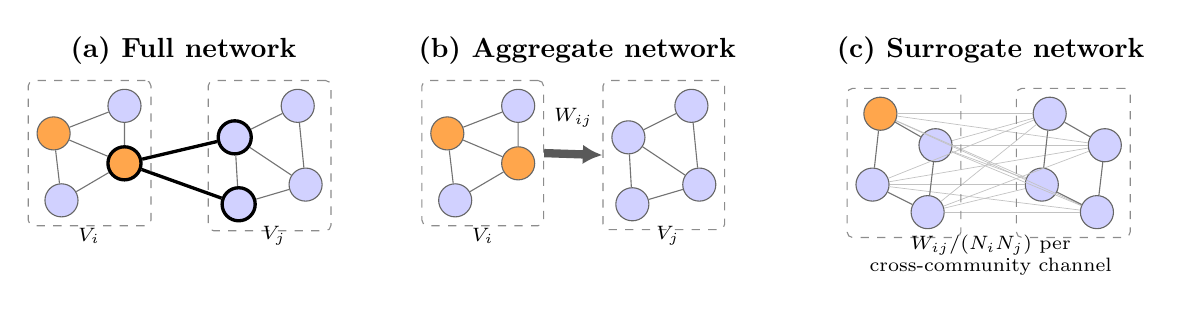
\begin{tikzpicture}[
  x=1cm,y=1cm,
  font=\scriptsize,
  >=Latex,
  person/.style={circle,draw=black!60,fill=blue!18,minimum size=4.2mm,inner sep=0pt},
  infected/.style={person,fill=orange!70},
  bridge/.style={person,very thick,draw=black},
  bridgeinf/.style={infected,very thick,draw=black},
  commbox/.style={draw=black!45,dashed,rounded corners=2pt,inner sep=3pt},
  macrobox/.style={draw=black!70,rounded corners=2pt,fill=black!5,align=center,inner sep=3pt},
  link/.style={draw=black!55},
  weak/.style={draw=black!24,line width=.25pt},
  flow/.style={-{Latex[length=1.7mm]},draw=black!65}
]
% (a) Full microscopic interface
\node[font=\bfseries] at (0,2.25) {(a) Full network};
\node[infected] (a1) at (-1.65,1.20) {};
\node[person]   (a2) at (-1.55,0.35) {};
\node[bridgeinf](a3) at (-0.75,0.82) {};
\node[person]   (a4) at (-0.75,1.55) {};
\node[bridge]   (b1) at (0.65,1.15) {};
\node[person]   (b2) at (1.45,1.55) {};
\node[person]   (b3) at (1.55,0.55) {};
\node[bridge]   (b4) at (0.70,0.30) {};
\draw[link] (a1)--(a2)--(a3)--(a1) (a1)--(a4)--(a3);
\draw[link] (b1)--(b2)--(b3)--(b4)--(b1) (b1)--(b3);
\draw[very thick] (a3)--(b1);
\draw[very thick] (a3)--(b4);
\node[commbox,fit=(a1)(a2)(a3)(a4)] {};
\node[commbox,fit=(b1)(b2)(b3)(b4)] {};
\node at (-1.2,-0.10) {$V_i$};
\node at (1.15,-0.10) {$V_j$};

% (b) Aggregate community network with local contacts retained
\node[font=\bfseries] at (5.0,2.25) {(b) Aggregate network};
\node[infected] (e1) at (3.35,1.20) {};
\node[person]   (e2) at (3.45,0.35) {};
\node[infected] (e3) at (4.25,0.82) {};
\node[person]   (e4) at (4.25,1.55) {};
\node[person]   (f1) at (5.65,1.15) {};
\node[person]   (f2) at (6.45,1.55) {};
\node[person]   (f3) at (6.55,0.55) {};
\node[person]   (f4) at (5.70,0.30) {};
\draw[link] (e1)--(e2)--(e3)--(e1) (e1)--(e4)--(e3);
\draw[link] (f1)--(f2)--(f3)--(f4)--(f1) (f1)--(f3);
\node[commbox,fit=(e1)(e2)(e3)(e4)] (agg_i) {};
\node[commbox,fit=(f1)(f2)(f3)(f4)] (agg_j) {};
\draw[-{Latex[length=2.5mm,width=2.5mm]},draw=black!65,line width=3pt]
      (agg_i.east) -- node[above=5pt,text=black] {$W_{ij}$} (agg_j.west);
\node at (3.8,-0.10) {$V_i$};
\node at (6.15,-0.10) {$V_j$};

% (c) Surrogate interface
\node[font=\bfseries] at (10.25,2.25) {(c) Surrogate network};
\node[infected] (c1) at (8.85,1.45) {};
\node[person]   (c2) at (8.75,0.55) {};
\node[person]   (c3) at (9.55,1.05) {};
\node[person]   (c4) at (9.45,0.20) {};
\node[person]   (d1) at (11.00,1.45) {};
\node[person]   (d2) at (10.90,0.55) {};
\node[person]   (d3) at (11.70,1.05) {};
\node[person]   (d4) at (11.60,0.20) {};
\foreach \u in {c1,c2,c3,c4}{\foreach \v in {d1,d2,d3,d4}{\draw[weak] (\u)--(\v);}}
\draw[link] (c1)--(c2)--(c4)--(c3)--(c1);
\draw[link] (d1)--(d2)--(d4)--(d3)--(d1);
\node[commbox,fit=(c1)(c2)(c3)(c4)] {};
\node[commbox,fit=(d1)(d2)(d3)(d4)] {};
\node[align=center] at (10.25,-0.35) {$W_{ij}/(N_iN_j)$ per\\cross-community channel};
\end{tikzpicture}
\caption{\textcolor{black}{Three views of the interface. (a) In the full network, infection can cross only through the shown physical edges and their bridge nodes. (b) Internal nodes and contacts are retained in each community. Individual inter-community contacts are represented by one wide directed edge between $V_i$ and $V_j$, labelled with their total weight $W_{ij}$. (c) The ideal two-scale process is equivalent to a process on a surrogate network with uniform inter-community connections: for each connected community pair, all ordered node pairs have the same contact weight. The connections together have total weight $W_{ij}$. Orange nodes are infected and blue nodes are susceptible.}}
\label{fig:schematic}
\end{figure}

\subsection{Local simulators}
\label{sec:local}

Each community has a separate Gillespie simulator for its local graph $G_i$. It applies the infection and removal rates in~\eqref{eq:full_generator} using only the local edges $E_{ii}$. The implementation updates only rates affected by the latest event, following \citet{kuryliak2025simulating}. Each local simulator is independent and has its own random-number stream.

The macro layer can advance a local simulator to a specified time. The simulator applies the local events up to that time. The macro layer can then import an infection by changing one selected susceptible node to $I$. This changes the local rates. The implementation keeps the unused part of the random threshold for the next local event and recalculates its waiting time using the new total rate.

To recalculate the time of the next local event after an import, the simulator retains the remaining random threshold. Let $E_{\mathrm{loc}}\sim\mathrm{Exp}(1)$ be the threshold drawn after the previous local event, and let $A_{\mathrm{loc}}$ be the integral of the total local rate from that event to the import time. After the import, the total local rate is $a_{\mathrm{new}}$. If $a_{\mathrm{new}}>0$, the remaining waiting time is
\[
\Delta t=
\frac{E_{\mathrm{loc}}-A_{\mathrm{loc}}}{a_{\mathrm{new}}}.
\]
Thus, an import changes the waiting time, but not the random threshold itself. If another import occurs first, the accumulated rate is updated and the waiting time is recalculated again. If $a_{\mathrm{new}}=0$, no local event can occur until the rate becomes positive.

The event type and its node are selected using the updated rates. A new local threshold is drawn only if there is no existing one. Each local clock has its own threshold, separate from the macro threshold described in Section~\ref{sec:timing}. For prescribed import times and target nodes, the local simulator follows the CTMC rules of its own network. The approximation comes from the way imports are generated and their target nodes are selected.

\subsection{Macro layer}
\label{sec:macro}

The macro layer represents each community by its current fractions and represents each directed connection by $W_{ij}$. Its rate for an infection from community $i$ to community $j$ is
\begin{equation}
\label{eq:macro_rate}
\lambda_{ij}(t)=\beta_{\mathrm{out}}W_{ij}\ibar_i(t)\sbar_j(t),
\qquad
\Theta(t)=\sum_{i\neq j}\lambda_{ij}(t).
\end{equation}
The factors have a direct meaning: $\beta_{\mathrm{out}}W_{ij}$ gives the total connection strength, $\ibar_i$ is the infected fraction in the source, and $\sbar_j$ is the susceptible fraction in the receiving community. The sum $\Theta$ is the rate of any cross-community infection. Calculating the waiting time to the next event when $\Theta$ varies with time requires special treatment (Section~\ref{sec:timing}).

When such an event occurs, first select the source and receiving communities $(i,j)$ with probability $\lambda_{ij}/\Theta$. Then choose one susceptible node uniformly in the receiving community $j$ and infect it. If there are 20 susceptible nodes, each has probability $1/20$. This selection does not use real bridge nodes, because the aggregate interface does not know them. In later formulas, we write this target probability as $\Pi_{ij}(v\mid x)=1/s_j$ for $v\in S_j$, where $x$ is the current network state. Thus, $\Pi$ simply denotes the probability of choosing a particular susceptible node. Other target rules can be used if bridge-node information is available.

This aggregate rate is generally an approximation to transmission through the real physical edges. For fixed community counts, it is the expected rate under uniformly random selection of the edge endpoints, before their particular identities, states, and epidemic history are taken into account. This does not guarantee the correct rate for an epidemic already realised on specific edges. For uniform all-to-all coupling, it is the actual rate, as explained in Section~\ref{sec:analysis}.

\subsection{Timing and synchronisation}
\label{sec:timing}

After a macro event at time $t_0$, draw a random threshold $E\sim\Exp(1)$: an exponential random number with mean one. Starting from zero, accumulate the total macro rate $\Theta$:
\begin{equation}
\label{eq:hazard_integral}
A(t)=\int_{t_0}^{t}\Theta(s)\,ds,
\qquad A(t_0)=0.
\end{equation}
The next macro event occurs at the first time $t^\ast$ when $A(t^\ast)=E$.

In words, the area under the rate curve grows until it first reaches the random threshold. If it never reaches the threshold, no further macro event occurs. This is the standard cumulative-rate construction \citep{ethier1986,anderson2007}. If $\Theta$ is constant, the waiting time is $E/\Theta$. Drawing $E=-\ln U$, with $U$ uniform on $(0,1)$, gives the familiar Gillespie waiting time. When $\Theta$ changes after a local event, we keep the same threshold and continue accumulating with the new rate. We draw a new macro threshold only after a macro event. Exact calculation of its first crossing defines the ideal process; the time-grid calculation below approximates that crossing. Section~\ref{sec:surrogate} shows that the ideal process is exact for the surrogate network with uniform inter-community connections.

The scheduler divides time into intervals of length $\tau$. On each interval, it approximates the varying macro rate by its value at the midpoint. Let $A$ be the amount already accumulated since the previous macro event. For the current interval $[t,t_g)$, copy every local simulator, including its random-number state, and advance each copy to the midpoint. The copies give an estimate $\Theta_{\mathrm{mid}}$ of the total macro rate. The estimated increase over the remaining interval is $\Theta_{\mathrm{mid}}(t_g-t)$. If $A$ plus this increase is below $E$ (the random macro threshold), the real simulators move to $t_g$. Otherwise, estimate the event time by
\begin{equation}
\label{eq:interpolation}
t^\ast=t+\frac{E-A}{\Theta_{\mathrm{mid}}}.
\end{equation}
Here, $E$ is the random macro threshold and $A$ is the amount already accumulated toward it. The numerator $E-A$ is what remains; dividing by the estimated rate gives the remaining waiting time. For example, if $E=1$, $A=0.4$, and $\Theta_{\mathrm{mid}}=0.2$, the estimated wait is three time units. The scheduler advances the real simulators to $t^\ast$, selects the source and receiving communities using their states at that time, chooses the susceptible target, and imports the infection. Algorithm~\ref{alg:scheduler} gives the full sequence.

\begin{algorithm}[tbp]
\color{black}
\caption{\textcolor{black}{Grid-synchronised two-scale simulation of one realisation.}}
\label{alg:scheduler}
\small

\textbf{Input:} local graphs $G_i$, weights $W_{ij}$, rates, step $\tau$, horizon $T_{\mathrm{end}}$, and initial state.
\begin{enumerate}
\item Set $t=0$ and accumulated rate $A=0$; draw $E\sim\Exp(1)$.
\item While $t<T_{\mathrm{end}}$ and infection can still spread, set $t_g=\min(t+\tau,T_{\mathrm{end}})$ and process the interval up to $t_g$.
\item Copy every local simulator, including its random-number state. Advance the copies to the midpoint of the remaining interval and calculate $\Theta_{\mathrm{mid}}$ from~\eqref{eq:macro_rate}.
\item If $A+\Theta_{\mathrm{mid}}(t_g-t)<E$, advance the real simulators to $t_g$, add this amount to $A$, set $t=t_g$, and return to step 2.
\item Otherwise, calculate $t^\ast$ from~\eqref{eq:interpolation} and advance the real simulators to $t^\ast$.
\item Select $(i,j)$ with probability $\lambda_{ij}(t^\ast)/\Theta(t^\ast)$. Select $v$ uniformly from $S_j(t^\ast)$ and import infection at $v$. Update the receiving local simulator, keeping its unused exponential threshold and selecting the local event from the new rates.
\item Set $t=t^\ast$ and $A=0$, draw a new $E\sim\Exp(1)$, and process the rest of the current interval in the same way.
\end{enumerate}

\end{algorithm}

The copied random-number states are important. Unless an import occurs first, a copied simulator follows the same path that the real simulator will follow to the midpoint. The midpoint estimate is exact on an interval with no local event. Its timing error and its look-ahead of at most $\tau/2$ decrease to zero as $\tau$ decreases.

The time grid is needed because the scheduler treats local simulators as black boxes. If they also report their next local-event times, the scheduler can merge those times and accumulate the piecewise-constant value of $\Theta$ exactly. That event-driven version removes the numerical synchronisation approximation. The experiments in this article use the implemented grid version with $\tau=1$.

\subsection{Computational structure and intended use}
\label{sec:cost}

\Full{} stores all local and cross-community channels, and its work per event grows with node degree \citep{kuryliak2025simulating}. \TS{} stores the local graphs and an $M\times M$ matrix of aggregate weights. The conference paper discusses this reduction in the information stored for cross-community contacts \citep{kuryliak2025towards}. Its importance depends on the problem. Replacing many individual cross-community edges by one weight can reduce storage. If only a few such edges exist, this saving may be small, and the local graphs still have to be stored.

The separate local simulators also provide an opportunity for parallel execution. Once the scheduler has chosen the next target time ($t_g$ or $t^\ast$), the local simulators can advance independently to that same time. The midpoint copies can also be processed in parallel. The macro layer must then collect the counts and apply any scheduled import before continuing. The implementation studied here advances the local simulators sequentially; parallel execution within one run is a possible extension, not a measured speedup. Local simulators can also use different community-specific settings.

The grid scheduler adds work by copying local states and coordinating the communities. Therefore, neither lower memory use nor faster execution is guaranteed. The method is useful when individual cross-community contacts are unavailable or too numerous to represent explicitly.


% English translation of the current Ukrainian main, active Sections 1--4.
% Translation of active Section 4 in the current Ukrainian main.
\section{Theoretical analysis of the two-scale method}
\label{sec:analysis}

The previous section described the two-scale simulation algorithm. The remaining question is how closely its results represent infection spread in the original network. Although the local simulators reproduce the within-community processes exactly, the macro layer uses aggregate connections instead of individual inter-community edges.

In this section, we first identify the network that mathematically corresponds to the ideal two-scale process. This establishes what changes when contacts are aggregated and separates these changes from the numerical synchronisation error. We then investigate how losing information about bridge nodes affects the first transmission time and introduce a characteristic for analysing accuracy in the experiments.

\subsection{Equivalence to simulation on a network with uniform inter-community connections}
\label{sec:surrogate}

The two-scale method replaces explicit inter-community contacts with aggregate infection rates while retaining exact stochastic dynamics within communities. This raises the question of whether the resulting process can be represented as exact simulation on a contact network and, if so, what that network looks like.

To answer this question, consider the ideal two-scale process, in which the time of each macro event is determined exactly by~\eqref{eq:hazard_integral}, without the time-grid approximation. This process is a continuous-time Markov chain (CTMC), because its transition rates depend on the current system state. Local transitions have the same rates as in the full-network model, while inter-community infections are determined by the aggregate rates~\eqref{eq:macro_rate} and the recipient-node selection rule.

We show that, when the susceptible recipient node is selected uniformly, this process is equivalent to exact simulation on a surrogate network with uniform inter-community connections, $\tilde G$ (Figure~\ref{fig:schematic}c). In this network, the total weight of each inter-community connection is distributed equally among all node pairs in the corresponding communities.

\begin{proposition}[Equivalence for a network with uniform inter-community connections]
\label{prop:surrogate}
Let $\tilde G$ have the same within-community contacts and their rates as the original network $G$. Replace each inter-community bundle $E_{ij}$ with the full set of channels $V_i\times V_j$, assigning each channel $(u,v)$ the rate
\[
\tilde\beta_{uv}
=
\frac{\beta_{\mathrm{out}}W_{ij}}{N_iN_j},
\qquad u\in V_i,\;v\in V_j,\;i\neq j.
\]
If the simulator selects the import target uniformly among susceptible nodes, the ideal two-scale process has the same rates for all transitions as the full-network process on $\tilde G$. Thus, from the same initial state, its distribution coincides with that of full-network Gillespie on $\tilde G$.
\end{proposition}

\begin{proof}
Local infections and removals have the same rates in both processes. It therefore suffices to compare the inter-community infection rates.

Consider any susceptible node $v\in V_j$ in system state $x$. In the two-scale process, imports from community $i$ to $j$ occur at rate $\lambda_{ij}(x)$, and the probability of selecting node $v$ is $1/s_j(x)$. Its total infection rate from other communities is therefore
\[
\begin{aligned}
\sum_{i\neq j}\lambda_{ij}(x)\frac{1}{s_j(x)}
&=
\sum_{i\neq j}
\beta_{\mathrm{out}}W_{ij}
\frac{y_i(x)}{N_i}
\frac{s_j(x)}{N_j}
\frac{1}{s_j(x)}
\\
&=
\sum_{i\neq j}
\sum_{u\in V_i}
\frac{\beta_{\mathrm{out}}W_{ij}}{N_iN_j}
\ind\{x_u=I\}.
\end{aligned}
\]

The last expression is the total infection rate of node $v$ through all inter-community channels of the surrogate network $\tilde G$ that lead to it from infected nodes. If $s_j(x)=0$, the community has no susceptible nodes, and inter-community infection is impossible in both models.

Thus, the rates of all possible transitions coincide. The generators of the two CTMCs are therefore identical, giving the same process distribution from the same initial state.
\end{proof}

\begin{corollary}
\label{cor:exact}
If every node in community $i$ is already connected to every node in community $j$ in the original network, and all these channels have the same rate for a given community pair, then $\tilde G=G$. In this case, the ideal two-scale method is also exact for the original network.
\end{corollary}

The ideal two-scale method therefore has an exact network interpretation: it reproduces the process on $\tilde G$. In general, however, the original and surrogate networks differ. The established equivalence does not by itself guarantee similar simulation results on these networks. To identify possible reasons for discrepancies, we examine which properties of inter-community contacts are preserved by their replacement and which change.

\subsection{Mechanisms of discrepancy from the full-network model}
\label{sec:sources}

By construction, the surrogate network $\tilde G$ preserves within-community contacts and the total coupling rate between each community pair:
\[
\sum_{(u,v)\in V_i\times V_j}\tilde\beta_{uv}
=
\beta_{\mathrm{out}}W_{ij}.
\]

This equality concerns the total rate of all channels, however, rather than only those through which infection can be transmitted in the current system state. The actual infection rate depends on the endpoint states of each contact. Equal total inter-community weights therefore do not guarantee the same infection dynamics.

Replacing real inter-community contacts by averaged connections changes three things: the transmission rate, the recipient node, and the possible number of imports. A fourth source of error is the approximate calculation of event times in the implementation.

\paragraph{1. The states of the real bridge nodes are not used.}
In the full network, the transmission rate from $V_i$ to $V_j$ is
\begin{equation}
\label{eq:exact_rate}
a^\star_{ij}(x)=\beta_{\mathrm{out}}\sum_{(u,v)\in E_{ij}}w_{uv}\,\ind\{x_u=I,\,x_v=S\},
\end{equation}
Only contacts from infected nodes to susceptible nodes contribute to this sum. If all bridge nodes in the source are still susceptible, transmission is impossible. In the two-scale method, the rate depends on the overall infected fraction, so infection of any source node can contribute to export. The method can transmit infection before any real bridge node is infected. We refer to this as \emph{bridge bypass} (Section~\ref{sec:single_export}).

The aggregate rate does not necessarily exceed the actual rate. If infected nodes are concentrated at the inter-community interface, the opposite can occur. Comparing rates in an individual state is therefore insufficient to establish the overall direction of a shift in transmission time.

\paragraph{2. Import location.}
In the full network, infection reaches the endpoint of the contact through which it was transmitted. The two-scale method selects any susceptible node with equal probability.
As a result, infection may reach a node that has no incoming contact from the corresponding source community in the original network. The location of the first infection affects subsequent spread within the community, including the time taken to reach bridge nodes leading to further communities. Changing the import-placement rule can therefore affect both local dynamics and infection spread through a sequence of communities.

\paragraph{3. Additional inter-community infections.}
In the SI model, each node can move from $S$ to $I$ only once. Each directed channel in the original network can therefore cause at most one infection of its target node. Consequently, at most $|E_{ij}|$ such infections can occur through the bundle $E_{ij}$.

The two-scale method does not track individual inter-community channels. After the first import, the rate $\lambda_{ij}$ can remain positive as long as the source community has infected nodes and the recipient community has susceptible nodes.

For example, if the communities are connected by just one directed channel, it can cause at most one infection in the full network. In contrast, \TS{} can import infection into several different nodes of the recipient community. These additional infections can accelerate internal spread and subsequent transmission to other communities.

\paragraph{4. Numerical synchronisation error.}
As described in Section~\ref{sec:timing}, the scheduler estimates the rate from the system state at the midpoint of a synchronisation interval and uses it to approximate the integral~\eqref{eq:hazard_integral}. The implemented \TS{} can therefore differ even from the ideal two-scale process on $\tilde G$.

% Ukrainian editorial note retained for review: is this remark needed?
\begin{remark}[The first import with randomly placed contacts]
\label{rem:placement}
Suppose that the endpoints of inter-community channels are selected uniformly and independently of the internal graphs and other contact sets, as in our tests. If the recipient community is still fully susceptible, the target of its first import is also uniform in the full network, after averaging over random contact placement. The two-scale method has the same distribution of the first target. For an individual fixed network, the targets need not coincide. The same distribution of the first target does not imply the same distribution of the first import time. Our tests show small errors in a number of configurations where the spread of internal infection times is small compared with the mean transmission time through one inter-community channel (Section~\ref*{sec:res_descriptor}).
\end{remark}

Replacing inter-community contacts thus changes not only the nodes through which infection can be transmitted, but also the possible locations and number of infections. These mechanisms can act simultaneously and should not be treated as independent additive components of the total error. Analysing them alone does not establish either the overall direction or the magnitude of discrepancies between the models.

\subsection{Effect of contact aggregation on systematic shifts in export time}
\label{sec:single_export}

We now examine how replacing individual inter-community contacts with an aggregate connection affects the first transmission time to another community. In particular, we ask whether aggregation can systematically shift the first export time even when the mean transmission rate is preserved.

To isolate the effect of losing information about bridge nodes, consider a simplified network: a connected source community $V_0$ with $n$ nodes and one external susceptible node $\ell$, called a leaf. The leaf is connected to a set $B\subset V_0$ of $k$ bridge nodes, with each channel having rate $\beta_{\mathrm{out}}$. The source follows SI dynamics, and the leaf does not affect internal infection spread before it becomes infected.

In the full-network model, the leaf can become infected only after at least one real bridge node becomes infected. In \TS{}, the aggregate coupling weight is $W_{0\ell}=k$, so before the leaf is infected, the export rate is
\[
\lambda_{0\ell}(t)
=
\beta_{\mathrm{out}}k\ibar_0(t).
\]
The possibility of export in the two-scale model therefore depends on the overall number of infected source nodes, rather than the states of the individual bridges.

Consider the case in which the $k$ bridge nodes are selected uniformly and independently of the internal dynamics. This allows us to compare first-export-time distributions while accounting for random placement of inter-community contacts.

\begin{proposition}[Stochastic ordering of the first export time]
\label{prop:ordering}
Let the bridge set $B$ be chosen uniformly from all $k$-element subsets of $V_0$, independently of the internal graph, initial state, and event randomness. Let $T^{\Full}$ and $T^{\TS}$ be the first infection times of the leaf in the full-network and ideal two-scale models, respectively. Then
\[
\mathbb{P}(T^{\Full}>t)
\geq
\mathbb{P}(T^{\TS}>t),
\qquad t\geq 0.
\]

Thus, with randomly placed bridges, the first export time in \TS{} is stochastically no greater than the corresponding time in \Full{}. The same ordering holds for its expectation and quantiles.
\end{proposition}

\begin{proof}
Before the leaf becomes infected, infection spread within $V_0$ is independent of external transmission. Both models can therefore be compared using the same internal SI trajectory $X_0$ of the source community.

Let $\tau_u$ be the infection time of node $u$, and let $A_u(t)=\max\{t-\tau_u,0\}$ be the time it has spent infected by time $t$.

In the full-network model, the cumulative export rate up to time $t$ is determined only by infected bridge nodes:
\[
H_B(t)
=
\beta_{\mathrm{out}}\sum_{u\in B}A_u(t).
\]

In \TS{}, the corresponding cumulative rate is determined by all source nodes:
\[
\bar H(t)
=
\beta_{\mathrm{out}}\frac{k}{n}
\sum_{u\in V_0}A_u(t).
\]

With a uniform, independent choice of $B$, each source node has probability $k/n$ of belonging to the bridge set. Conditional on the trajectory $X_0$, therefore,
\[
\mathbb{E}_B[H_B(t)\mid X_0]
=
\bar H(t).
\]

The cumulative rate in \TS{} is thus the expected cumulative rate in \Full{} over random bridge placement. Equality of these quantities does not, however, imply equality of the export-time distributions.

The probability of no export by time $t$ is the exponential of the negative cumulative rate. Since $z\mapsto e^{-z}$ is convex, Jensen's inequality gives
\[
\begin{aligned}
\mathbb{P}(T^{\Full}>t\mid X_0)
&=
\mathbb{E}_B[e^{-H_B(t)}\mid X_0]
\\
&\geq
e^{-\mathbb{E}_B[H_B(t)\mid X_0]}
\\
&=
e^{-\bar H(t)}
\\
&=
\mathbb{P}(T^{\TS}>t\mid X_0).
\end{aligned}
\]

Because this inequality holds for every internal trajectory $X_0$, it also holds after averaging over all possible trajectories, proving the proposition.
\end{proof}

This result shows that the aggregate rate matches the expected actual rate, yet the transmission-time distributions can differ systematically. The reason is the nonlinear dependence of the probability of no event on the cumulative rate: averaging rates is not equivalent to averaging the corresponding probabilities.

In addition to shifting time, aggregation can violate constraints on admissible transmission routes. Let $T_B=\min_{u\in B}\tau_u$ be the infection time of the first real bridge node. In the full-network model, the leaf cannot become infected before $T_B$. In ideal \TS{}, however, the probability of such an early export is
\begin{equation}
\label{eq:bypass}
\mathbb{P}(T^{\TS}<T_B)
=
\mathbb{E}\left[
1-\exp\left(
-\beta_{\mathrm{out}}\frac{k}{n}
\int_0^{T_B}y_0(s)\,ds
\right)
\right].
\end{equation}

This expression gives the probability that the aggregate rate causes an export before any real bridge node becomes infected. It shows that even when export-time distributions are close, the two models can differ in whether their transmission paths are admissible.

For randomly placed bridges, we have therefore established the direction of the stochastic shift in the first export time, but not its magnitude. The next question is which properties of internal spread make this discrepancy small or substantial.

% The former Section 4 temporal-descriptor drafts are commented out in the
% Ukrainian source; the active descriptor is now in Section 5 below.

\section{Methodology for experimental evaluation}
\label{sec:design}

\subsection{Experimental networks and parameters}

The theoretical analysis in the previous section showed how aggregating inter-community contacts changes infection transmission and under which conditions a stochastic shift in the first export time arises. However, it does not determine the magnitude of the discrepancies between the models or their behaviour after successive inter-community crossings.

To investigate these questions, we compare \Full{} and \TS{} in four experimental series. We first consider transmission to a single external node and then infection spread along a chain of communities. In each setting, we examine how internal network structure affects the discrepancies between the models.

All experiments use SI dynamics, unit contact weights, $\beta_{\mathrm{in}}=\beta_{\mathrm{out}}=\beta$, and a synchronisation step of $\tau=1$ (Algorithm~\ref{alg:scheduler}).

\paragraph{Clique--leaf.}
To compare the first export times of the two methods with minimal influence from internal network structure, we use a complete graph. The receiving community need not be represented in full: for this purpose, it is sufficient to represent export through the bridge nodes and a single external leaf.

We attach one external node (the leaf) to a complete graph (clique) with $n=100$ nodes through $k=2$ distinct bridge nodes in the clique. We perform 10\,000 runs of each model with $\beta=0.005$ and a time horizon of 1000. In this and all other experiments, bridge nodes are selected uniformly without replacement.

\paragraph{Random community--leaf.}
We next investigate how the internal structure of the source affects infection transmission to the leaf. We replace the clique with a connected random graph of $n=1000$ nodes and attach the leaf through $k\in\{1,5\}$ distinct bridge nodes.

We characterise internal structure by the average shortest-path length (ASPL). To generate the graph, we first construct a uniformly random tree and then add random edges to obtain the target ASPL within a tolerance of 0.1. We vary ASPL from 1 to 6 in steps of 0.25; ASPL 1 corresponds to a complete graph.

As ASPL increases, the mean degree of the generated graphs also decreases. This experiment therefore investigates the effects of internal path length and network sparsity.

The initially infected node is selected uniformly from all source nodes. For each configuration, we perform 400 runs of each model: 40 realisations of the internal graph with 10 replicates of inter-community contacts and random events. We use $\beta=0.003$ and a horizon of 30\,000.

\paragraph{Chain of cliques.}
The preceding tests consider just one inter-community crossing. To examine how discrepancies change after successive crossings, we connect $L=10$ complete graphs, each with $n=1000$ nodes, in a line, with one edge between neighbouring communities ($k=1$). Infection starts in community 0.

As in the first test, complete graphs provide rapid internal spread. This allows us to assess the effect of successive inter-community crossings in a baseline setting with minimal internal path lengths.

We use $\beta=0.003$, 400 runs of each model, and a horizon of 30\,000.

\paragraph{Chains of random communities.}
Finally, we combine successive inter-community crossings with variation in internal community structure. This series examines how community size and internal structure affect discrepancies between \Full{} and \TS{}, and how these discrepancies change along the chain.

We connect $L=10$ connected random communities in a line, with $k\in\{1,5\}$ edges between neighbouring communities. Infection starts in community 0.

We consider sizes $n\in\{50,100,250,1000\}$. Internal graphs are generated by the procedure described above, varying ASPL from 1 to 6 in steps of 1.

For each interface, we select $k$ nodes uniformly without replacement from each community and connect them in pairs. A node can participate in interfaces with both neighbouring communities.

For each configuration, we perform 400 runs of each model with $\beta=0.003$ and a horizon of 30\,000. Two \Full{} runs were extended to 40\,000 to observe infection of the last community (Appendix~\ref*{app:repro}).

\begin{table}[tbp]
\centering
\caption{Parameters of the experimental series. ASPL is the target average shortest-path length within a community.}
\label{tab:design}
\small
\begin{tabular}{
>{\raggedright\arraybackslash}p{0.17\linewidth}
>{\raggedright\arraybackslash}p{0.36\linewidth}
>{\raggedright\arraybackslash}p{0.06\linewidth}
>{\raggedright\arraybackslash}p{0.08\linewidth}
>{\raggedright\arraybackslash}p{0.20\linewidth}}
\toprule
Series & Structure & $k$ & $\beta$
& Runs per cell and model \\
\midrule
Clique--leaf
& Clique $n=100$ and one leaf
& 2 & 0.005 & 10\,000 \\

Random community--leaf
& $n=1000$, ASPL 1--6 in steps of 0.25,
one leaf
& 1, 5 & 0.003 & 400 (40 $\times$ 10) \\

Chain of cliques
& $L=10$, $n=1000$
& 1 & 0.003 & 400 (40 $\times$ 10) \\

Chains of random communities
& $L=10$, $n\in\{50,100,250,1000\}$,
ASPL 1--6 in steps of 1
& 1, 5 & 0.003 & 400 (40 $\times$ 10) \\
\bottomrule
\end{tabular}
\end{table}

Each pair of \Full{} and \TS{} runs uses the same internal graphs, inter-community contacts, and initially infected node, but independent streams of random events. Inter-community contacts are generated independently for different interfaces and replicates.

\subsection{Metrics for comparing the models}

To assess discrepancies between \Full{} and \TS{}, we compare infection propagation times and cases of transmission before the bridge nodes become infected.

In the leaf tests, we measure its first infection time $T_{\mathrm{export}}$. For chains, let $T_c$ be the first infection time of community $c$, where $c=1,\ldots,9$. Since the chain has 10 communities, the arrival time in the last community is denoted by $T_9$.

Because infection spread is stochastic, the time of the same event varies between runs. The first infected nodes and infection paths also differ between runs. Comparing individual realisations is therefore insufficient to assess discrepancies between the models.

For each configuration, we perform repeated runs of \Full{} and \TS{}. Each run yields one time for the corresponding event: infection of the leaf or the first infection of a particular community. From these values, we form separate empirical distributions for the two models and compare them using three metrics.

\paragraph{Relative median shift.}
To determine how much earlier or later \TS{} transmits infection than \Full{}, we calculate the relative difference between the medians of the corresponding distributions:
\[
b_c =
100\,
\frac{
\operatorname{med}(T_c^{\TS})-
\operatorname{med}(T_c^{\Full})
}{
\operatorname{med}(T_c^{\Full})
}.
\]
A negative value means earlier infection arrival in \TS{}, while a positive value means later arrival. The median shift describes the direction and magnitude of the difference in typical times, but does not describe the whole distribution.

\paragraph{Normalised Wasserstein distance.}
The median shift captures only the difference between the medians and does not account for the rest of the distribution. To assess differences between empirical distributions of event times, we therefore use the Wasserstein-1 distance.

We sort the $R$ observed times of the corresponding event in ascending order separately for each model and calculate
\[
W_1 =
\frac{1}{R}
\sum_{r=1}^{R}
\left|
T_{(r)}^{\TS}-T_{(r)}^{\Full}
\right|,
\]
where $T_{(r)}^{\TS}$ and $T_{(r)}^{\Full}$ are the $r$th values in the ordered \TS{} and \Full{} samples, respectively.

To compare results with different characteristic propagation times, we normalise the distance by the mean time in \Full{}:
\[
\eW =
100\,\frac{W_1}{\overline{T}^{\Full}}.
\]
The resulting measure describes the difference between empirical distributions independently of the direction of the shift. The formula compares ordered samples, not individual pairs of runs.

In the leaf tests, both metrics are calculated for $T_{\mathrm{export}}$; in chains, they are calculated for the arrival times $T_c$.

\paragraph{Fraction of premature exports}
Similar infection-time distributions do not guarantee that an admissible sequence of infection transmission is preserved. In the full network, infection cannot reach a neighbouring community until at least one real bridge node in the source becomes infected. In contrast, \TS{} can transmit infection before any of these nodes becomes infected.

To assess how often this occurs, for each inter-community crossing we consider the set $B$ of real bridge nodes in the source community. Let $\tau_u^{\TS}$ be the infection time of node $u$ in the corresponding \TS{} run. The infection time of the first bridge is then
\[
T_B^{\TS}=\min_{u\in B}\tau_u^{\TS}.
\]

Let $T_{\mathrm{arr}}^{\TS}$ be the first infection time of the recipient community or leaf. We record a premature export if
\[
T_{\mathrm{arr}}^{\TS}<T_B^{\TS}.
\]

The fraction of premature exports is the percentage of such cases among all examined inter-community crossings in \TS{}. This metric describes how often a necessary condition for transmission through real bridge nodes is violated.

\paragraph{Discrepancies along the chain.}
For chains, we additionally compare the relative shifts in the mean durations of the first crossing, $T_1$, and the subsequent crossings, $T_9-T_1$. The first crossing allows us to assess discrepancies associated with export from the initial community, while later crossings can also reflect the effects of import placement and surplus imports. This comparison tests whether discrepancies become stronger after the first inter-community crossing.

\subsection{A measure of the ratio of time scales}
\label{sec:descriptor}

Discrepancies between \Full{} and \TS{} may depend not only on network structure, but also on the relative speeds of infection spread within and between communities. In particular, aggregation does not account for when individual bridge nodes become infected, which can matter when internal spread is slow and uneven.

To investigate this relationship, we use the dimensionless measure
\begin{equation}
\label{eq:rho}
\rho=\beta_{\mathrm{out}}\sigma_T,
\end{equation}
where $\sigma_T$ is the standard deviation of node infection times within a community. This measure describes the spread of internal infection times relative to the mean transmission time through one continuously active inter-community channel, $1/\beta_{\mathrm{out}}$.

For each configuration, we calculate $\sigma_T$ from node infection times in each source community of the \Full{} runs, then average these values over communities and runs.

We examine how $\rho$ relates to the median shift and normalised Wasserstein distance for the arrival time in the last community, $T_9$. In particular, we compare how well $\rho$ and ASPL explain discrepancies between the models across community sizes and structures.

A small $\rho$ means that the spread of internal infection times is small relative to the transmission time through one channel. We test whether such configurations show smaller discrepancies between the models.

For each configuration, $\sigma_T$ is calculated from node infection times in the source communities of the \Full{} runs and averaged over these communities and runs.

In the results, we compare $\rho$ with the median shift and normalised Wasserstein distance across community sizes, internal structures, and numbers of inter-community edges.

The measure $\rho$ is not a direct error metric. We consider it a possible explanatory characteristic of the discrepancies. Since $\sigma_T$ is calculated from \Full{}, we do not test whether error can be predicted from local simulations alone.

% User's Ukrainian editorial note: not sure whether this subsection is needed.
\subsection{Statistical evaluation}

Because the simulations are stochastic and the number of runs is limited, the estimated discrepancies between \Full{} and \TS{} have sampling uncertainty. We use a block bootstrap to assess this uncertainty and a permutation test to test differences between infection-time distributions.

\paragraph{Block bootstrap.}
Replicates on the same graph share its structure and are therefore not independent realisations of a network configuration. To account for this dependence, the bootstrap samples whole network blocks with replacement, keeping all ten replicates and their corresponding pairs of \Full{} and \TS{} runs together.

For chain summary statistics, we form 2000 bootstrap samples and recalculate the measures of interest. The limits of the 95\% confidence intervals are the 2.5th and 97.5th percentiles of the resulting estimates. This assesses uncertainty in the magnitude and direction of discrepancies between the models.

\paragraph{Permutation test.}
The Wasserstein distance can be positive even for two samples from the same distribution, because each contains a finite number of random observations. We therefore need to test whether the observed distance exceeds the level that can arise from sampling variability.

For each pair of runs, we randomly swap the observed \Full{} and \TS{} infection times with probability $1/2$. We recalculate the normalised Wasserstein distance from the resulting samples. Repeating this procedure 2000 times gives a distribution of distances under random reassignment of results between models.

Under the null hypothesis that \Full{} and \TS{} results are exchangeable within pairs, we use this distribution to assess the statistical significance of the observed distance. Its 95th percentile defines the permutation threshold, and the fraction of permutations with a distance at least as large as the observed one estimates the $p$-value.

Exceeding the threshold indicates a statistically significant discrepancy under the assumed null model.

% User's Ukrainian editorial note: not sure whether this subsection is needed.
\subsection{Validation of the Full implementation}

To validate the full-network simulator, we compare the simulated mean infection time of the first bridge node, $T_B$, with the analytical value for a clique (Appendix~\ref*{app:clique}). This check uses four clique sizes and two numbers of inter-community edges.

We also check the mean transmission time to the leaf after the single bridge becomes infected. For one continuously active channel, its theoretical value is $1/\beta$.

These checks assess the agreement of the \Full{} implementation with known analytical results, but do not establish the accuracy of the two-scale approximation.


\bibliographystyle{cas-model2-names}
\bibliography{twoscale_references}
\end{document}
